\documentclass[slidetop,11pt]{beamer}

\usepackage[utf8]{inputenc}
\usepackage[frenchb]{babel}
\usepackage{verbatim}
\usepackage{graphicx}
\usetheme{Warsaw}

\AtBeginSection[]
{
  \begin{frame}<beamer>
    \frametitle{Syllabus}
        {\scriptsize\tableofcontents[currentsection,hideothersubsections]}
  \end{frame}
}

\title{Projet d'ALN}
\author{Lemarchand Benoit \\ Megna Anaël \\ Shimi Adam}
\institute{ENSEEIHT}
\date{Lundi 1 juin 2015}

\begin{document}

%%%%%%%%%%%%%%%%%%%%%%%%%%%%%%%%%%%%%%%%%%%%%%%%%%
\frame{\titlepage}


%%%%%%%%%%%%%%%%%%%%%%%%%%%%%%%%%%%%%%%%%%%%%%%%%%
\section{Travail algorithmique}
\begin{frame}
  \frametitle{}
  \begin{itemize}
    \item Implémenter la subspace iteration method.
    \item Utiliser le sous-espace significatif pour la reconstruction.
    \item Trouver le sous-espace significatif le plus proche d'une observation
          pour la classification.
  \end{itemize}
\end{frame}


%%%%%%%%%%%%%%%%%%%%%%%%%%%%%%%%%%%%%%%%%%%%%%%%%%
\section{Test du code Fortran}
\begin{frame}
  \frametitle{}
  \begin{figure}
  \begin{center}
    \caption{temps relatif en fonction de n et p}
    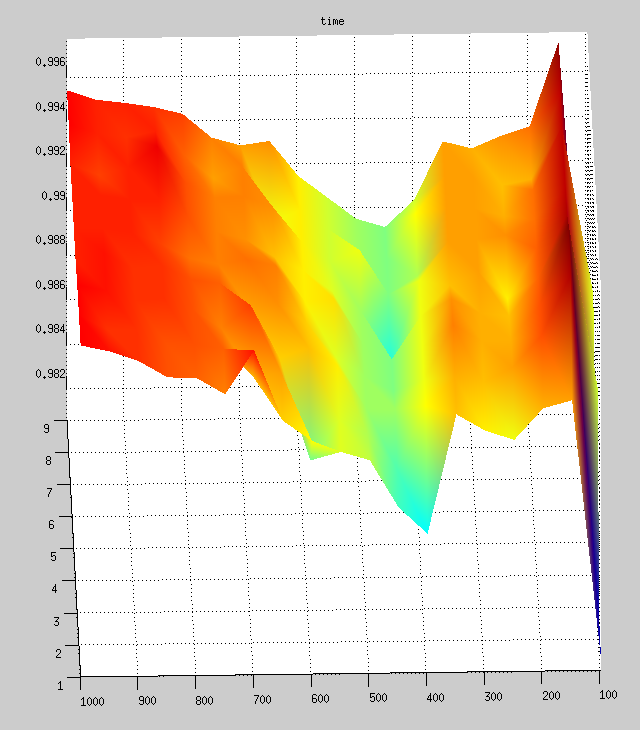
\includegraphics[width=5cm]{imat4.png}
  \end{center}
  \end{figure}
\end{frame}


%%%%%%%%%%%%%%%%%%%%%%%%%%%%%%%%%%%%%%%%%%%%%%%%%%
\section{Test du code Matlab}
\begin{frame}
  \frametitle{}
  \begin{figure}
  \begin{center}
    \caption{temps relatif en fonction de Nens et percentInfo}
    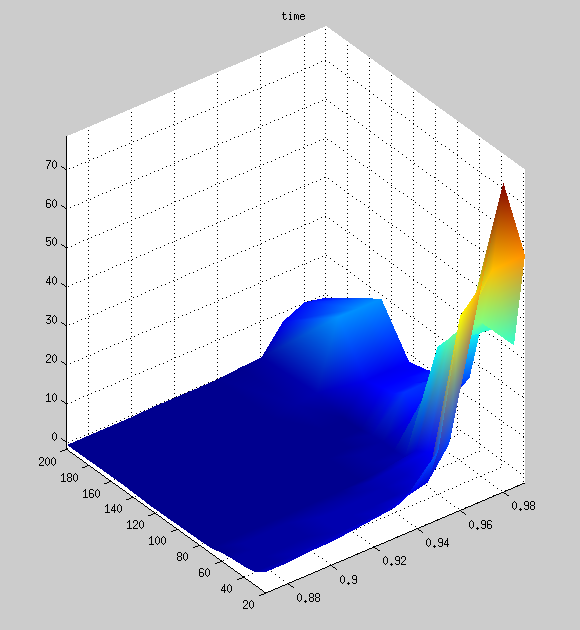
\includegraphics[width=5cm]{time1.png}
  \end{center}
  \end{figure}
\end{frame}


%%%%%%%%%%%%%%%%%%%%%%%%%%%%%%%%%%%%%%%%%%%%%%%%%%
\section{Prise en compte du modèle physique}
\begin{frame}
  \frametitle{}
  \begin{figure}
  \begin{center}
    \caption{temps relatif en fonction de Nens et percentInfo}
    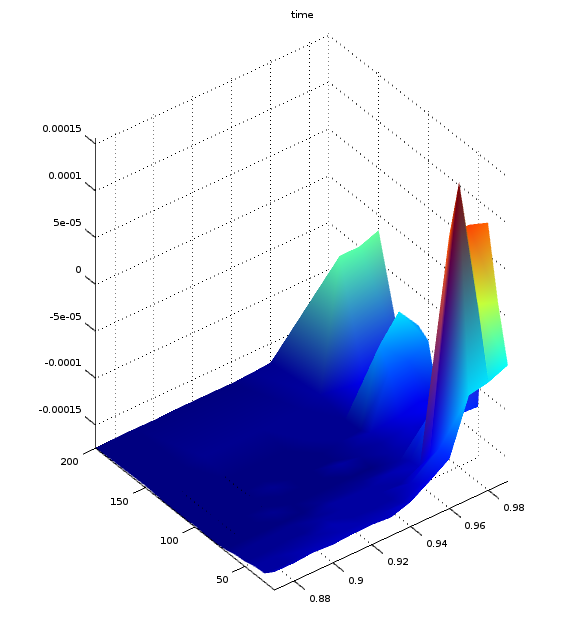
\includegraphics[width=5cm]{time2_1.png}
  \end{center}
  \end{figure}
\end{frame}
\begin{frame}
  \frametitle{}
  \begin{figure}
  \begin{center}
    \caption{erreur relative en fonction de Nens et percentInfo}
    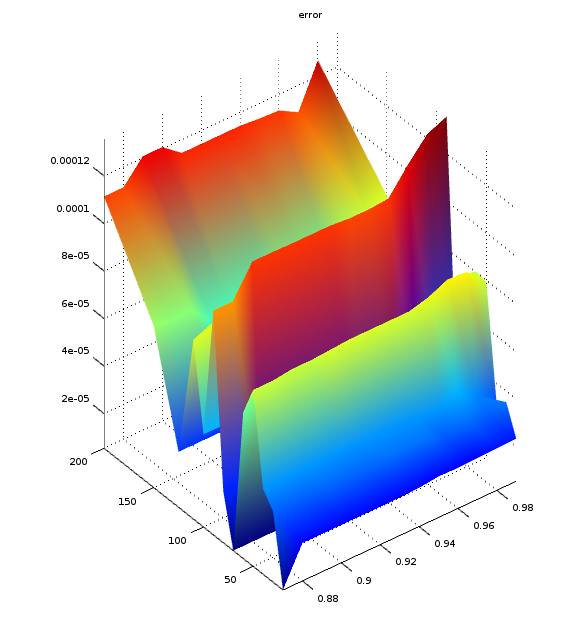
\includegraphics[width=5cm]{error2_1.png}
  \end{center}
  \end{figure}
\end{frame}

\end{document}
